\section{\emph{rag}, a Ruby Autograder for ESaaS}

Having chosen Ruby and Rails for their excellent testing and
code-grooming tools, our approach was to repurpose those same tools into
autograders that would give finer-grained feedback than human graders
using more detailed tests, and would be easier to repurpose than
those built for other languages.

\begin{figure}
  \begin{tabular}{|p{0.15\textwidth}|p{0.15\textwidth}|p{0.7\textwidth}|}
 \hline
 \textbf{Grader} & \textbf{Based on} & \textbf{Student Assignment Type} \\
 \hline
 RSpecGrader &
 unit testing &
 Student submits one or more class files; black-box and ``intrusive''
 unit tests against functions and groups of functions are performed
 \\
 FeatureGrader &
 simplified mutation testing &
 Student submits integration tests written using Cucumber; bugs inserted
 in reference app attempt to trigger test failures to check test suite
 completeness and test fragility
 \\
 MechanizeGrader & 
 staging-like integration testing &
 Student deploys full-stack app to public cloud; ``black box'' tests
 stimulate remote server and parse/analyze output, including execution
 of JavaScript if needed
 \\
 \hline
\end{tabular}

  \caption{\label{fig:grader_summary} Summary of the autograder
    engines based on our repurposing of excellent existing open-source
    tools and testing techniques.  Only the RSpecGrader is
    Ruby-specific; the others are easily retargetable to other languages
    and systems.}
\end{figure}

\texttt{rag}\uf{github.com/saasbook/rag} 
is actually a collection of three different autograding
``engines'' based on open-source testing
tools, as Figure~\ref{fig:grader_summary} shows.  
Each engine takes as input a student-submitted work
product and one or more rubric files, and grades the work according to
the rubric.  The contents of the rubric files depend on the type of
engine used.\footnote{Currently the rubric files must be present in the
  local filesystem of the autograder VM, but refactoring is in progress
  to allow these files to be securely loaded on-demand from a remote
  host so that currently-running 
  autograder VMs do not have to be modified when an assignment is added
  or changed.}
The first of these is
\textbf{RSpecGrader}, based on RSpec, an XUnit-like 
TDD framework that exploits Ruby's
flexible syntax to embed a highly readable unit-testing DSL in Ruby.
The instructor annotates specific tests within an assignment with point
values (out of 100 total); RSpecGrader computes the total points
achieved and concatenates and formats the error/failure messages from
any failed tests, as Figure~\ref{fig:rspec_grader_rubric} shows.
RSpecGrader  runs RSpec in a separate timer-protected interpreter
thread in which large sections of the
standard library such as file I/O and most system calls have been
stubbed out, allowing us to handle exceptions in RSpec itself as well
as test failures.  

\begin{figure}
  \centering
    \lstinputlisting[numbers=left,tabsize=1,basicstyle=\scriptsize\ttfamily]{figs/rspec_grader_rubric.rb}
  \caption{\label{fig:rspec_grader_rubric}
    In an RSpecGrader rubric, some test cases are ``sanity checks''
    without which the assignment isn't even graded
    (lines 2--9) while others contribute points to the
    student's score.  Ruby's dynamic language features allow us to
    easily check, for example, that
a student's implementation of a ``sum all the numbers'' method does not
simply call a built-in library method (line 7).
  }
\end{figure}

A variant of RSpecGrader is \textbf{MechanizeGrader}.
Surveys of recent
autograders~\cite{ihantola-2010-autograding-survey,douce-2005-autograding-survey}
mentioned as a ``future direction'' a grader that can assess full-stack
GUI applications.
MechanizeGrader does this using Capybara and
Mechanize\footnote{\url{jnicklas.github.io/capybara},
\url{rubygems.org/gem/mechanize}}.
Capybara provides a Ruby-embedded DSL for interacting with Web-based
applications by providing primitives that trigger actions on a web page
such as filling in form fields or clicking a button, and examining the
server's delivered results pages using XPath\uf{w3.org/TR/xpath20/}, as
Figure~\ref{fig:mechanize_grader_example} shows. 
Capybara is usually used as an in-process testing tool, but Mechanize
can trigger Capybara's actions against a remote application, allowing
black-box testing.
Students' ``submission'' to MechanizeGrader is therefore the URL to their
application deployed on the public 
cloud.  (We use the free tier of Heroku for our assignments and
projects.)

\begin{figure}
 \centering
  \lstinputlisting[language=Ruby,numbers=left]{figs/mechanize_grader_example.rb}
  \caption{\label{fig:mechanize_grader_example} 
This excerpt of three test cases from a MechanizeGrader rubric runs
against a student's 
deployed full-stack application.}
\end{figure}

Finally, one of our assignments requires students to write integration-level
tests using Cucumber, which allows such tests to be formulated in
stylized plain text, as Figure~\ref{fig:cucumber} shows.
Our autograder for this
style of assignment is inspired by mutation testing, a technique invented
by George Amman and Jeff 
Offutt~\cite{ammann-offutt-sw-testing} in which a
testing tool pseudo-randomly mutates the program under test to ensure
that some test fails as a result of these introduced errors.

\begin{figure}
  \centering
    \lstinputlisting{figs/cucumber_example.feature}
    \lstinputlisting[language=Ruby]{figs/cucumber_step_def_example.rb}%
  \caption{\label{fig:cucumber} Cucumber accepts integration tests 
    written in stylized prose (top) and uses regular expressions to map each
    step to a \emph{step definition} (bottom) that sets up preconditions, exercises the app,
    or checks postconditions.  Step definitions 
    can stimulate a full-stack GUI-based web application in various
    ways, including remote-controlling a real browser with Webdriver
    (formerly Selenium) or using the Ruby Mechanize library to interact
    with a remote site.  Our code blocks are in Ruby, but the Cucumber framework
itself is polyglot.} 
\end{figure}

Specifically, \textbf{FeatureGrader} operates by working with an
existing application to which student-created tests will be applied.   The application is modified so that the FeatureGrader
can adjust the application's behavior by manipulating certain environment variables. Each  scenario 
specified by the assignment is first tested against the working application.  Assuming the 
students have created the correct acceptance tests in Cucumber, all these tests should pass.  

Next the FeatureGrader starts to mutate the underlying application
according to a simple specification (Figure~\ref{fig:featuregrader}), running the specified feature against
the mutated application and checking that the specified scenarios do in fact fail.  Students 
lose points according to the weights associated with features that do not generate the expected failure.


\begin{figure}
  \begin{minipage}{0.45\textwidth}%
  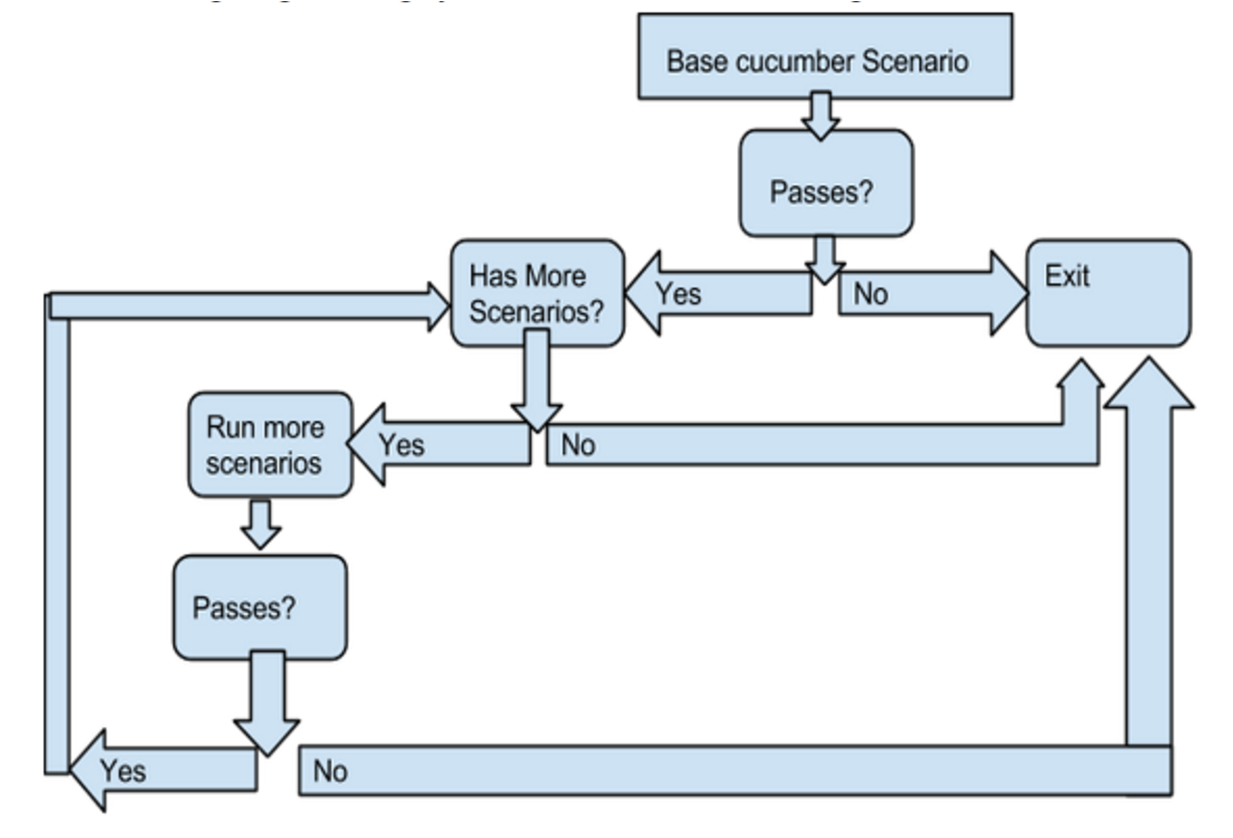
\includegraphics[width=\textwidth]{figs/feature_grader.pdf}%
  \end{minipage}%
  \begin{minipage}{0.55\textwidth}%
  \lstinputlisting{figs/feature_grader_example.yml}%
  \end{minipage}
  \caption{\label{fig:featuregrader}%
FeatureGrader workflow and example YAML file.  In this case if Step1-1 passes,
Step1-3 will be run next.  Earlier steps must be less restrictive than
later steps (if the earlier step fails, there should be no way that a later one could pass).
\texttt{failures} are the two student-provided Cucumber scenarios that \emph{should fail} when
run because of mutations (bugs) inserted in the app.
}
\end{figure}

